\chapter{PorthosC: The implementation}
\label{ch:impl}

The main call for commencing the work on \porthos[2] was the need for processing real-world C programs, which, at first, requires the input language to be extended.
This implies the support not only for new syntactic structures of the C language (such as the \texttt{switch} statement or the postfix increment operator \texttt{i++}), but also for its fundamental concepts and features (such as types, pointer arithmetic or first-order functions), which requires revision of the whole architecture of the tool.
Yet far from all the C language is supported (which, considering its complexity and numerous pitfalls, goes far beyond current thesis%
%
\footnote{To ensure this, one merely has to look at existing C compiler implementations, for instance, the open-source \tool{gcc} compiler, which uses the C parser written in more than 18.5 thousand lines of code (see \url{https://github.com/gcc-mirror/gcc/blob/master/gcc/c/c-parser.c})}%
%
), we consider the accomplished work as a step towards it.
%This applies not only to instances that simply constitute the syntactic sugar of C language (such as the \texttt{switch} statement or the prefix increment operator \texttt{++i}), but also to its fundamental concepts and features (such as pointer arithmetic or structures).
%However, the architecture of current version of \porthos{} does not allow to ... as it is ....
% Although and optimisation of the tool so that it is able to process real C programs in perspective.

%In current Chapter we discuss the new architecture of \porthos[2].

% function invocations/calls: inlining with binding
% contexts: for now, no ctxs
% comparing to cprover (https://www.cprover.org/cbmc/doc/manual.pdf, page 45, absatz about 'goto') where "the loop is unwound a given number of times" , we SHOULD have 2 modes of unrolling: 1) number of times, and 2) number of high-level instructions executed
% TODO(code): (https://www.cprover.org/cbmc/doc/manual.pdf, page 45) "The break and continue statements are replaced by equivalent goto statements as described in the ANSI-C standard."

% TODO: arrays: cprover manual page 48


%\section{The architecture of \porthos{}}
\section{General principles}
\label{ch:impl:principles}

The previous version of \porthos{} did not distinguish the event-based program model from the high-level AST, they both were encoded into a single SMT-formula (see classes of package `\texttt{dartagnan.program}' of \porthos[1]).
%For 
Moreover, the syntax tree was implemented as a mutable data structure, which is being modified at all stages of the program (for instance, see the methods `\texttt{dartagnan.program.Program.compile(...)}' of \porthos{} that recursively compute some properties of the AST and change its state).
We are inclined to consider this architecture as one that is fast to develop, but hard to maintain (since it is difficult to guarantee the correctness of the program) and extend (since adding the support for a new high-level instruction requires changing multiple components of the program, from parser to encoder).
%Moreover, we encounter serious problems when we need to add support for control-flow jumps (as \texttt{continue}, \texttt{break}, \texttt{goto} in C).

Therefore, while working on the new design of \porthos[2], we decided to clearly separate the high-level intermediate code representation (an AST structure) from the low-level event-based representation (an event-flow graph).
Such a modular architecture will allow to support multiple input languages%
%
\footnote{Apart from the C language, \porthos[2] must be able to analyse litmus tests in different assembly languages and, as a compatibility mode, the input language of \porthos[1].} %
%
by parsing them and converting parsed syntax trees to a simplified AST.

All internal representations used by \porthos[2] must be immutable, so that it is possible to guarantee the correctness of the program by controlling its invariants.
The immutability in \porthos[2] is implemented via \texttt{final} fields that are assigned by the immutable-object values (either a primitive type, or another immutable object, or an immutable collection provided by the library Guava by Google%
%
\footnote{The Guava project repository: \url{https://github.com/google/guava/}}%
%
).

During the development of \porthos[2], we mainly followed the \textit{KISS~principle}, which can be exhaustively described in 17 Unix Rules of Eric Raymond~\cite{raymond2003art}.
The following list summarises the main rules we followed during the development of \porthos[2]:

\vspace{0.5em}
\begin{enumerate}[nolistsep]
  \item \textit{Robustness:}
    \begin{enumerate}[label*=\arabic*.]
      \item preservation the completeness of analysis,
      \item modular architecture: each module can be tested independently,
      \item usage of software design patterns where necessary, and
      \item usage of immutable data structures for all DTOs.
    \end{enumerate}
  \item \textit{Transparency:}
    \begin{enumerate}[label*=\arabic*.]
      \item following the principles of simplicity and readability,
      \item clear and informative program output, and
      \item following the clear code style.
    \end{enumerate}
  \item \textit{Efficiency:}
    \begin{enumerate}[label*=\arabic*.]%[leftmargin=1.5em]
      \item keeping the trade-off between execution time and memory usage.
    \end{enumerate}
  \item \textit{Extensibility:}
    \begin{enumerate}[label*=\arabic*.]%[leftmargin=1em]
      \item clear modular architecture.
    \end{enumerate}
\end{enumerate}

Robustness of the analysis is the main criterion of \porthos[2] as a verification tool.
Although it makes the analysis more sensitive to the combinatorial explosion, it preserves the completeness of analysis, which is necessary for a model-checking tool.
As a robust and transparent tool, \porthos[2] must adhere to the strategy of aborting its work on any unexpected outcome (for instance, if a parser failed to parse the string and the recovery algorithm is not described).
One of the transparency principles is following the clear code style.
This mainly means the clear and informative naming of classes, functions and fields.
It also implies the unified ordering of methods in classes, minimised size of methods code, clear tabulation, etc.
%The modular architecture of \porthos[2] allow each its module to be tested independently.
%Usage of immutable data structures for all DTOs helps 
%immut: preservation of invariants
%The transparency, efficiency and extensibility are the necessary criteria of any good tool.

As its predecessor, \porthos[2] uses the open-source SMT solver \tool{Z3}%
%
\footnote{The \tool{Z3} project repository: \url{https://github.com/Z3Prover/z3}} %
%
by Microsoft Research~\cite{de2008z3}. However, unlike its predecessor, \porthos[2] has an additional abstraction level, \zformula{} (see Section~\ref{ch:impl:model:zformula}), that allows the use any other SMT solver.

%We have decided to implement \porthos[2] in \textit{Java}
As its predecessor, \porthos[2] is written in \textit{Java},
%The programming language choice for \porthos[2] was also made in favour of \textit{java},
firstly, in order to be able to reuse some parts and concepts of \porthos{} also written in Java, and secondly, because the authors find the object-oriented (OOP) concepts of Java suitable for modelling languages.
Although Java does not show the best results in performance benchmarks (for example, compared to C++~\cite{hundt2011loop}), the performance cornerstone of \porthos[2] (as well as any other SMT-based code analyser) is the phase of solving the SMT-formula, which is left to the third-party SMT solver invoked by \porthos[2] via a Java API.
However, considering the perspective of using \porthos[2] as a static analyser for real-world programs, the memory optimisation problem must also be taken into account during both encoding and solving stages.
It is worth noting that, for the reasons of simplicity, \porthos[2] is not a concurrent program, however, we believe that, due to its modular architecture, it can be easily parallelised on the level of program modules.


\begin{figure}
  \centering
  %draft=true
  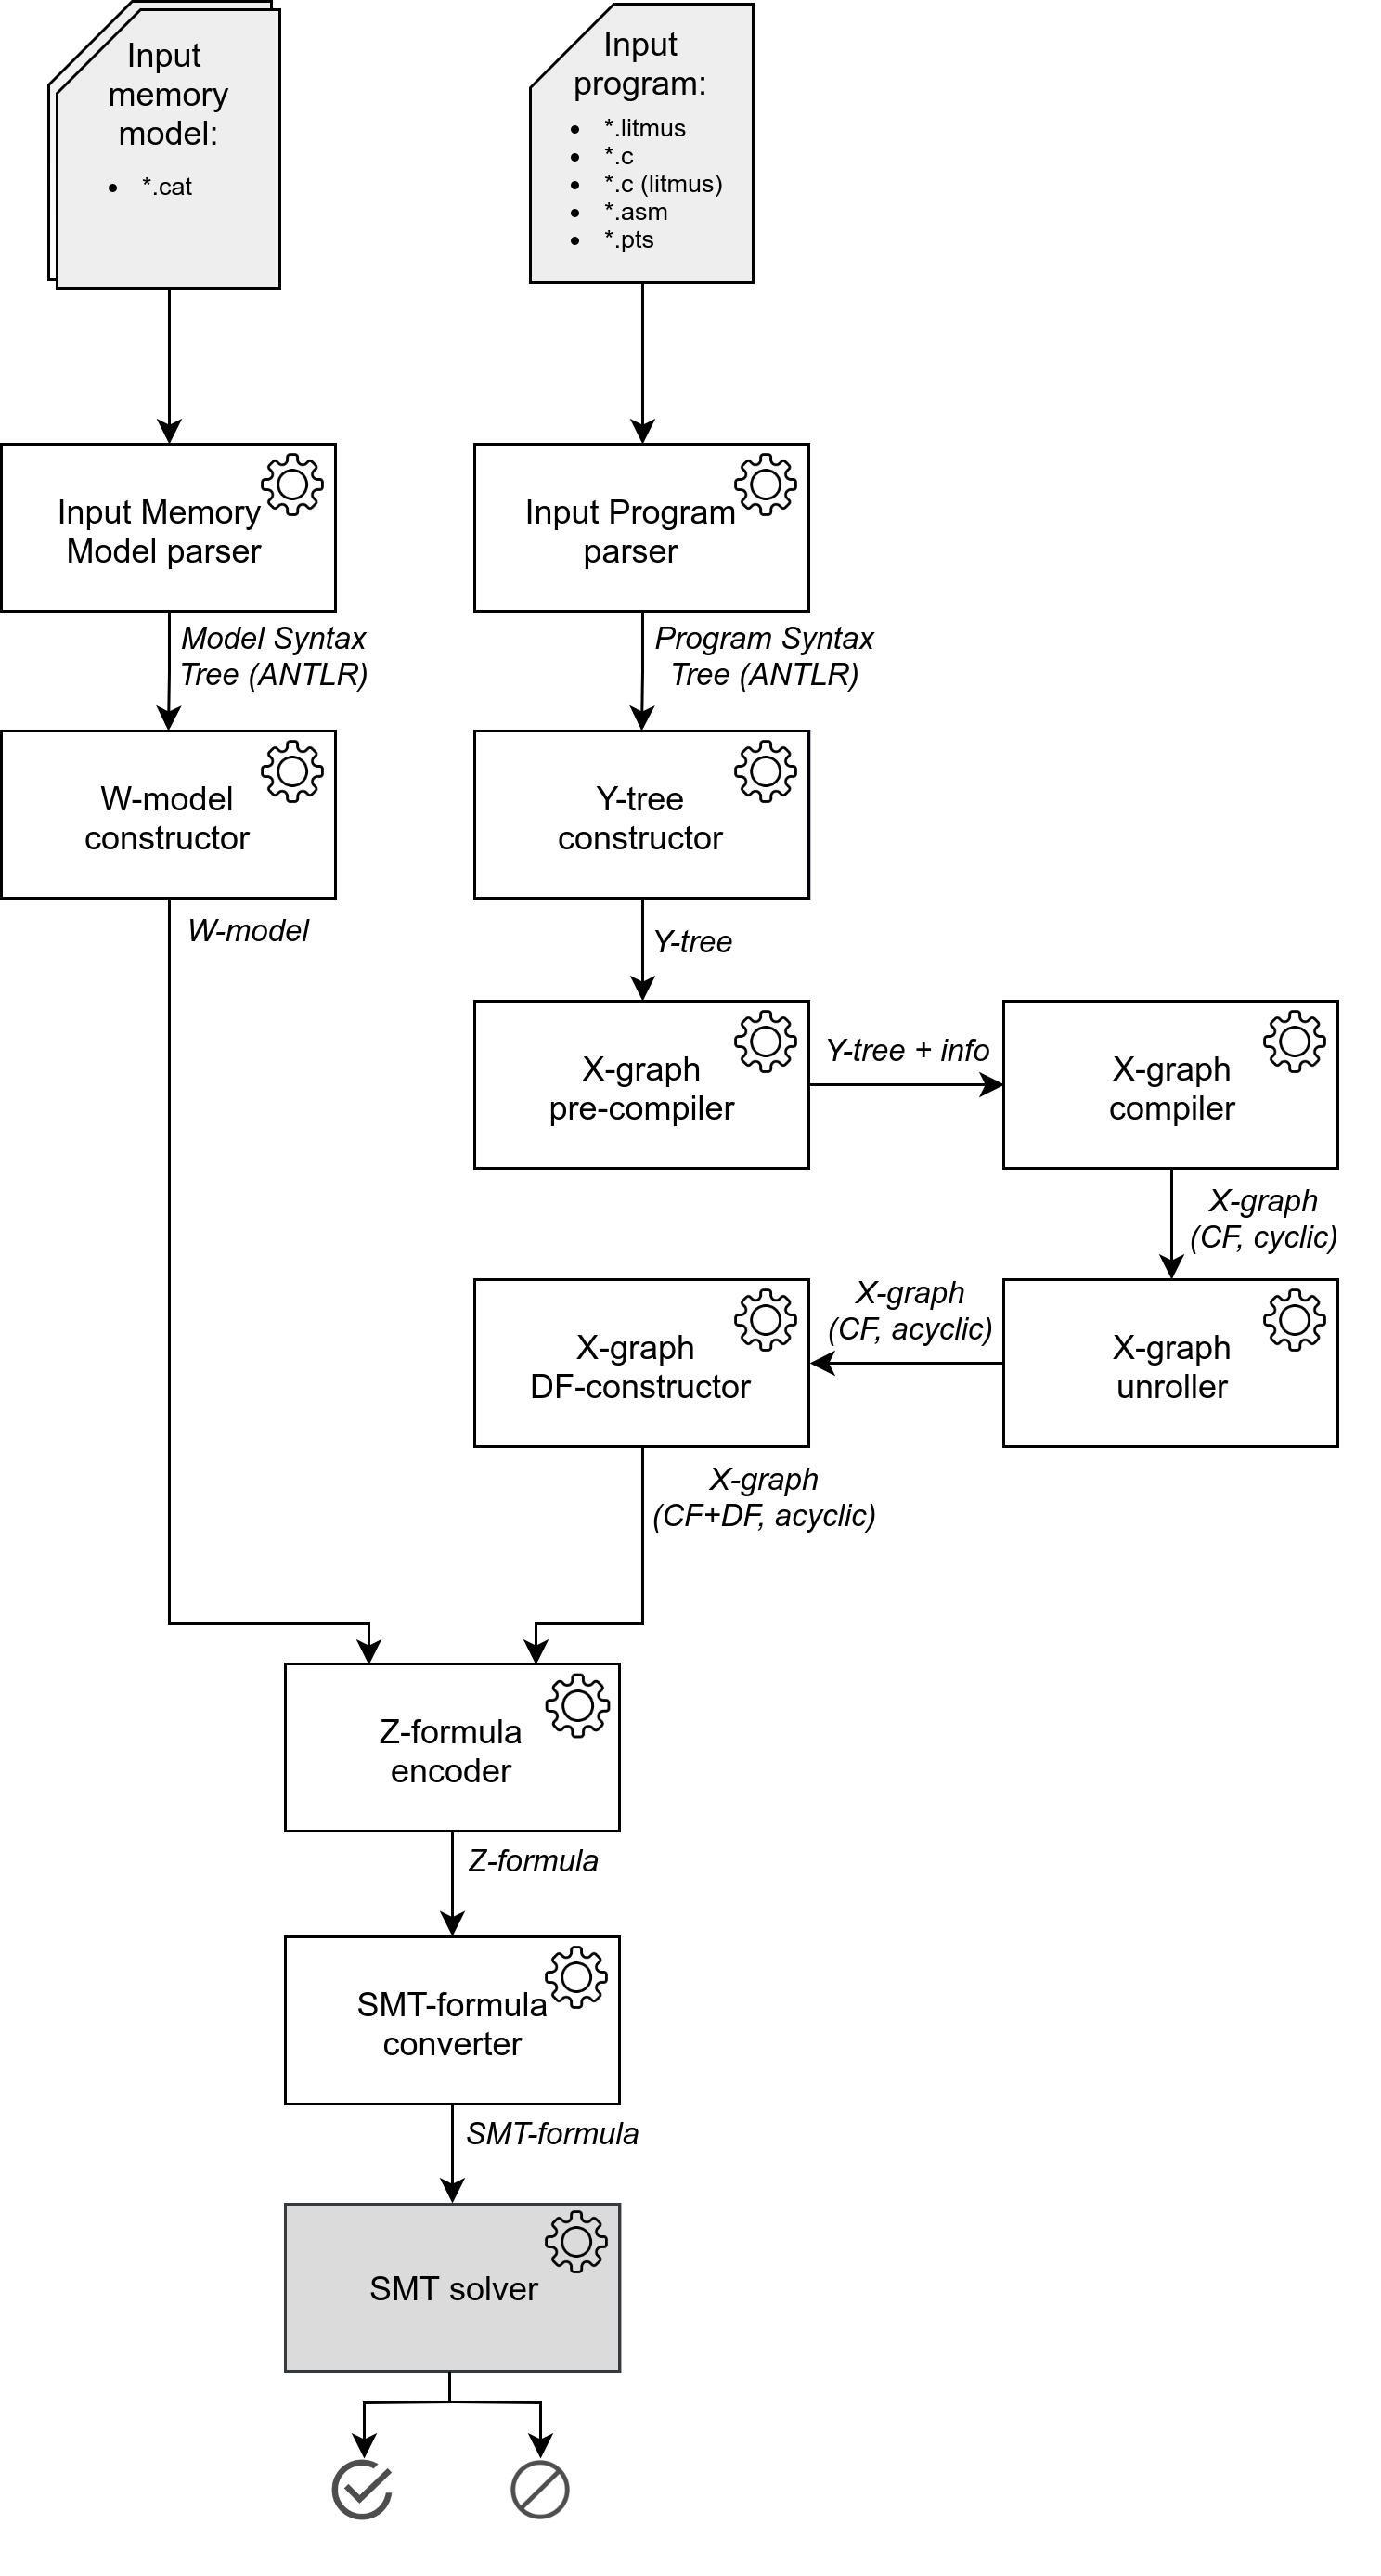
\includegraphics[height=.99\textheight,keepaspectratio]{img/my/draw.io/general_arch-no_numbering.png} %{img/my/draw.io/general_arch.png}
  \caption{The general architecture of \porthos[2]}
  \label{fig:arch}
\end{figure}

\section{The architecture}
\label{ch:impl:arch}

The general architecture scheme of \porthos[2] is presented in Figure~\ref{fig:arch}.
%The rectangles in the picture denote processing units (marked with gear sign with a unique number of the component), and labels of the arrows describe the internal representation carried out during the transformation.

The program takes as input the program to be analysed and one (the reachability analysis mode) or two (the portability analysis mode) memory models.
However, instead of parsing memory models from the \cat{} file, the tool may operate with pre-defined memory models (\texttt{SC}, \texttt{TSO}, \texttt{PSO}, \texttt{RMO}, \texttt{ALPHA}, \texttt{POWER}, \texttt{ARM}; this feature is inherited from \porthos[1]).
The parsed program syntax tree is then converted (Section~\ref{ch:impl:proc:y-constr}) to a program AST called \ytree{}%
%
\footnote{In order to avoid confusion between different internal representations, we prefix the names of elements of each internal representation with a letter. For instance, we picked the letter `Y' to denote the AST code representation as drawing of this letter resembles the tree branching; with letter `X' we prefix elements of the event-flow graph as the events are to be e\textbf{x}ecuted; and with letter `W' we prefix elements of the \textbf{w}eak memory model AST.}%
%
(Section~\ref{ch:impl:model:ytree}), which then is being preprocessed at the pre-compilation stage (Section~\ref{ch:impl:proc:x-pre-compiler}) in order to collect information necessary for the compilation.
The \ytree{} then is being compiled (Section~\ref{ch:impl:proc:x-compiler}) to an \xgraph{} representation (Section~\ref{ch:impl:model:xgraph}).
The compiled \xgraph{} then is being converted to an acyclic form (Section~\ref{ch:impl:proc:x-unroll}) in order to be encoded into a \zformula{} (Section~\ref{ch:impl:model:zformula}).
Apart from that, the memory-model constructor (Section~\ref{ch:impl:proc:w-constr}) constructs the abstract syntax tree of derived relations of the weak memory model \wmodel{} (Section~\ref{ch:impl:model:wmodel}).
%on the basis of the \xgraph{} in order to build the weak memory model \wmodel{} (Section~\ref{ch:impl:model:wmodel}).
Thereafter, \wmodel{} and acyclic \xgraph{} are encoded (Section~\ref{ch:impl:proc:z-encoder}) to a \zformula{} representation (a wrapper over an SMT-formula), which then is translated to an SMT-formula (Section~\ref{ch:impl:proc:smt-converter}), which then is solved by the SMT solver (Section~\ref{ch:impl:proc:smt-solver}).


\subsection{Program input}
\label{ch:impl:input}
%(for instance, the original input language of \porthos{} tool, two variants of syntax of a litmus test used by \tool{herd}, an assembly language for any supported architecture).

Both \porthos{} and \porthos[2] use the \tool{ANTLR} parser generator%
%
\footnote{The \tool{ANTLR} project repository: \url{https://github.com/antlr/antlr4}}%
%
~\cite{parr2013definitive}, a powerful language processing tool.
The \tool{ANTLR} takes as input the user-defined grammar of the target language in a BNF-like form and produces the LL(*)-parser and optionally some auxiliary classes (such as listeners and visitors for the syntax tree).
Although this parser may not be as efficient as a hand-written language-optimised parser, it reduces the overhead of implementing the parser significantly.
Among other advantages \tool{ANTLR}, it has a rather large collection of officially supported grammars.
Nonetheless, the intuitive syntax for defining grammars and numerous of tools for debugging grammars make the \tool{ANTLR} an attractive instrument for solving the parsing problem.

\begin{figure}[t]%[!h]%[!hb]
\centering
%basicstyle=\ttfamily\tiny,
\begin{lstlisting}[basicstyle=\rmfamily\scriptsize,%
  %alsoletter={:,|,;,(,)},
  %morekeywords={:,|,;,(,)},
  %keywordstyle=\color{dkblue},
  literate=%
  {<}{{$\langle$}}1
  {>}{{$\rangle$}}1,
  escapeinside={[*}{*]},]
<program>
      :      <initialisation>   <thread>+   <assertion>
      ;
<thread>   
      :      thread   <thread-id>   <instruction>
      ;
<instruction>
      :      <atom>
      |      `{'   <instruction>   `}'
      |      <instruction>   `;'   <instruction>
      |      `while'   `('   <bool-expr>   `)'   <instruction>
      |      `if'   <bool-expr>   `{'   <instruction>   `}'   <instruction>
      ;
<atom>   
      :      <register>   `[*<*]-'   <expression>
      |      <register>   `[*<*]:-'   <location>
      |      <location>   `:='   <register>
      |      <register>   `='   <location>   `.'   `load'      `('   <atomic>   `)'
      |      <location>   `='   <register>   `.'   `store'   `('   <atomic>   `)'
      |      (`mfence'   |   `sync'   |   `lwsync'   |   `isync')
      ;
<bool-expr>
      :      `true'
      |      `false'
      |      <expression>   (`and'      |      `or')   <expression>
      |      <expression>   (`=='   |   `!='   |   `>'   |   `>='   |   `[*<*]'   |   `[*>*]=')   <expression>
      ;
<expression>   
      :      [0-9]
      |      <register>
      |      <expression>   (`*'   |   `+'   |   `-'   |   `/'   |   `%')   <expression>
      ;
\end{lstlisting}
\caption{The sketch of the input language grammar used by \oldporthos}
\label{fig:in_grammar_pts}
\end{figure}

Figure~\ref{fig:in_grammar_pts} represents the grammar sketch in BNF syntax of the input language used by \porthos[1].
%(the full \tool{ANTLR} grammar is available at Appendix~\ref{apx:grammar}).
%TODO! Reformulate this.
The input language parser used by \porthos{} suffered from several disadvantages.
Firstly, it contained the parser code inlined directly into the grammar, so that the grammar would serve as a template for the parser code (which is called semantic actions).
Such a combining of two expressive languages makes the code hardly understandable and, therefore, poorly maintainable.
In \porthos[2], we clearly separated the parser (generated from the grammar file `\textit{<grammar>.g4}') from converting the \tool{ANTLR} syntax tree to the AST, that is one for all languages of an input program.

Secondly, \porthos{} resolved the semantics of operations syntactically (it was defined in the \tool{ANTLR} grammar), whereas it should be resolved by a separate module operating on the AST level%
%
%\footnote{Most modern languages (including C++) allow the function overloading, thus requiring the type information to be available for the function resolution algorithm (see Section~\ref{ch:impl:proc:x-pre-compiler}).}%
%
, so that it does not require to change grammar for encoding the semantics of a new function. %adding support for a new function.
%\footnote{for instance, given two functions `\lstinline{foo(int a)}' and `\lstinline{foo(char a)}' compiled by a C++ compiler, the code `\lstinline{int a = '1'; foo(a);}' will invoke the first method rather than the second one.}.%
As the reader may have noticed from the grammar sketch in Figure~\ref{fig:in_grammar_pts}, the memory operations of different kinds vary syntactically as well.
For example, the assignment of local computation to a register uses the symbol `\lstinline{<-}', the atomic non-relaxed load operation denoted as `\lstinline{<:-}', atomic non-relaxed store operation denoted as `\lstinline{:=}', and the semantics of relaxed \lstinline{load} and \lstinline{store} are resolved syntactically by matching the function name.
Moreover, only the operator `\lstinline{<-}' could have an expression as the source of data, which means that expressions could be assigned only to registers.
% (thus, the variable \lstinline{r} was recognised as a local variable as well).
In \porthos[2], the semantics of the data-flow operation is determined according to the types of operands, that are determined during the pre-compilation stage (see Section~\ref{ch:impl:proc:x-pre-compiler}).
The semantics of the functions also is being resolved during the pre-compilation stage via the \textit{invocation hooking} mechanism (see Section~\ref{ch:impl:proc:x-compiler}).

Thirdly, the grammar used by \porthos{} allowed only a restricted set of operations.
For example, it accepted the computation expressions only over local variables.
Thus, in the assignment expression `\lstinline{r <- (x + 1);}', the variable \lstinline{x} was parsed as a local variable even though it can be used as a shared variable in other parts of the program.
In \porthos[2], all shared variables involved into a computation expression are tentatively copied to temporary local variables.
%Moreover, expressions could be assigned only to local variables only via the assignment operator `\lstinline{<-}' (thus, the variable \lstinline{r} was recognised as a local variable as well).
%, which might lead to inconsistency of the result SMT-formula if the same variable name was used both as a register and as a location, for instance, the in code `\lstinline{x := reg1; reg2 <- (x + 1);}', the first statement interprets the variable \lstinline{x} as a location, while the grammar of second statement requires it to be a register.

Fourthly, \porthos[1] supported only integer constants and expressions.
%Also, only integers were processed by the input language parser of \porthos{}.
In \porthos[2], we extended support for primitive types supported by the \tool{Z3} solver (this apply to 32-bit integers encoded as \texttt{Int}s of \tool{Z3}, floats encoded as \texttt{Real}s, enumerations encoded as \texttt{Scalar}s).
%TODO : constant arrays? https://rise4fun.com/\tool{Z3}/tutorial/guide
Although the \tool{Z3} supports the array theory (characterised by the select-store axioms~\cite{de2011z3}), the complexity of pointer analysis for the arrays of non-constant size moves the full support of arrays and pointers out of the scope of current thesis.
%Thus, adding support for more advanced structures as pointers, arrays, function definitions and calls was one of the purposes of revising the tool architecture.

Finally, the grammar used by \porthos{} had the following minor drawbacks. %A minor drawback of 
The operators were implemented as non-associative (expressions of the form `\lstinline{1 + 2 * 3}' could not be parsed).
Comparing to C statements, that must end with the semicolon punctuator `\lstinline{;}', statements defined in the grammar of \porthos[1] use the semicolon as a separator between statements (the final statement must not end with semicolon).
The litmus-specific syntax for variables initialisation was used only for declaring the shared variables (all of them were initialised with default value \lstinline{0}), however, this syntax should be used as an initial assignment of both shared and local variables with arbitrary values.
%initialise them with a value different from the default \lstinline{0} or to initialise a local variable.
%did not allow to assign an arbitrary value to a variable (the default value \lstinline{0} was used).

%Also, \porthos{} supports only the litmus-specific syntax for the variables initialisation, however, it allows only initialisation of the shared variable and only by default value \lstinline{0}.
%\porthos[2] supports arbitrary declaration to be performed in initialisation statement.

\porthos[2] uses the C language grammar of proposed in the C11 standard~\cite{jtc2011sc22}, that was extended by litmus test-specific syntax such as initialisation and final-state assertion statements (the original \tool{ANTLR} grammar can be found in the official repository containing the collection of \tool{ANTLR v4} grammars%
%
\footnote{ANTLR grammars repository path:~\url{https://github.com/antlr/grammars-v4}}). %
%
Current version of \porthos[2] does not recognise C processor directives (it ignores them), however, in future it can be extended to support them.

Currently, \porthos[2] can operate only in the intra-procedural analysis mode, assuming that each function defined in the input file is being executed in a separate thread.
%TODO: describe more intra- and inter-procedural!
However, the redesigned architecture of \porthos[2] can be easily extended to support the inter-procedural (cross-procedure) analysis that inlines function calls and binds variable contexts.
%TODO : check in the implementation , THAT WE HAVE NOT IMPLEMENTED THIS FEATURE!!
Thus, instead of analysing a single source code file, the user can analyse the whole code project.
In this mode, the functions to be executed in parallel should be specified by the user.
Also, the tool may be extended to detect the concurrent parts of the code automatically at the pre-compilation stage.
For that, the pre-compiler should recognise functions that commence a new process (such as \texttt{pthread\_create} from \texttt{pthread.h}) and resolve the argument that points to the thread function.
This functionality %implies an additional stage of the pre-compilation and 
is left beyond current thesis.
%resolve the semantics of function invocations and remember the functions 
%function that commence new process or thread 
%(for instance, the function \texttt{pthread\_create} of the library \texttt{pthread.h} that starts the new thread of the function it received as the first argument).
%TODO: inter: user specifies the repository with code, functions that intended to work in parallel and runs. 

%TODO: say sth about 100500 litmus-tests for kernel


\subsection{Internal representations}
\label{ch:impl:model}

%Internal representations used in \porthos[1] 

%As it has already been mentioned, all internal representations used by \porthos[2] are immutable.
For keeping the architecture transparent, we build all abstraction levels with interfaces, even if some of them does not add any new functionality.% (as java does not support multiple inheritance for classes (only for interfaces), we 

\subsubsection{Y-tree}
\label{ch:impl:model:ytree}

The first internal representation used by \porthos[2] is the \textit{\ytree{}}, which represents a high-level recursively%
%
\footnote{Hereinafter we use the term \textit{recursive} data structure (sometimes called \textit{inductive}) to refer a complex data type which can contain elements that contain other elements of the same type.
For example, an unary expression contains references to the operator and the child expression of the same type.} %
%
defined AST.
The Apendix~\ref{apx:trees} presents the file tree of the main classes that constitute the \ytree{} hierarchy (as the inheritance tree might be obvious for the C-like AST, we confine ourselves to presenting the classes file tree only, which we tend to retain clearly structured).

%\columnratio{0.7}%\begin{paracol}{2}
%\switchcolumn%\VerbatimInput{inc/lst/Ytree-tree.out}%\end{paracol}
The abstract syntax tree, \ytree{}, is an abstraction level suitable for compiling the program to a low-level representation (in the case of processing low-level assembly code, it may be directly converted to the \xgraph{} representation).
In terms of \porthos[1], the \ytree{} is the level of \textit{instructions}.
%In contrast to \ytree{} representation, the \tool{ANTLR} syntax tree follows the same structure as the grammar, which is a superset of the real (meaningful) grammar of the C language.
%However, it lacks some concepts of the language (for example, the syntax of indexer access corresponds the grammar rule "\lstinline{postfixExpression '[' expression ']'}" for an arbitrary postfix %, that is converted to the \texttt{YIndexerExpression}).
However some details of the syntax might have been abstracted away (for instance, array operations may be emulated by functions invocations, see~\cite[Chapter 5]{gries2012science}), we find this level of abstraction suitable enough for modelling a high-level language.

Each \ytree{} element implements the interface \texttt{YEntity} and carries the \texttt{OriginLocation} %
%\textbf{(TODO: Rename CodeLocation->OriginLocation in the code!)} %TODO <--
instance that contains information about the coordinates of the input text that has generated the \ytree{} element.

Following the C11 standard~\cite{iso2012iec}, we distinguish a \textit{statement} (\textit{"an~action to be performed"}) from an \textit{expression} (\textit{"a sequence of operators and operands that specifies computation of a value, or that designates an object or a function, or that generates side effects, or that performs a combination thereof"}).

All \ytree{} expressions implement the \texttt{YExpression} interface.
On the \ytree{} level, the pointer arithmetic is modelled by the integer number \textit{pointer level} of an expression (although in fact this is the property of a type not of an expression, the y-tree is an untyped syntax tree, therefore the elements \ytree{} should carry this property).
We distinguish the subset of expressions that imply no side-effects, they implement the interface \texttt{YAtom} and can be global or local (which is defined also syntactically).
Each \ytree{} expression carries the original code coordinates, that can be resolved to text by the service \texttt{LocationService}. %todo: rename from CodeCitationService + create 3 instances for each of level. Or keep it for Y->text, and store references to the original Y-object by X-objects

%\textbf{(TODO:THIS SHOULD BE IN PRE-PROCESSING)} %TODO <--

\vspace{1em}
The \ytree{} expressions are the following:

\begin{itemize}%[nolistsep]
  \item \texttt{YBinaryExpression} that model the C binary operator (\textit{relative} operator that compares two expressions of any type, \textit{logical} that processes two boolean expressions, and \textit{numerical} that processes two numerical expressions);
  %\textbf{TODO: rename 'integer'->'numerical' in code} %TODO <--

  \item \texttt{YUnaryExpression} that model the C unary expression (logical negation, numeric prefix and postfix increment and decrement, bitwise complement);

  \item \texttt{YMemberAccessExpression} that has an arbitrary expression of type \texttt{YExpression} as its base expression (it will be resolved during the compilation stage);%TODO: pre-compilation??

  \item \texttt{YIndexerExpression} and \texttt{YInvocationExpression} that as arbitrary expression as its base or arguments (strictly speaking, the indexer expression is an unary-function invocation, but as the SMT solver we use supports the constant-array theory, we can maintain the array type);

  \item \texttt{YAssignmentExpression} that assigns an \texttt{YExpression} to an \texttt{YAtom};

  \item \texttt{YVariableRef} that stores the untyped "reference" to a variable (viz., the name only);

  \item \texttt{YLabeledVariableRef} that represents the litmus-specific local variable reference for a certain the process (e.g., `\lstinline{P0:x}' which means the local variable \lstinline{x} of the process \lstinline{P0});

  \item \texttt{YParameter} that represents a typed variable (the type was declared, similarly to the variable definition); and

  \item \texttt{YConstant} that represents an untyped non-named constant.
\end{itemize}

%\vspace{0.5em}
Similarly to expressions, all \ytree{} statements implement the \texttt{YStatement} interface. The statements are the following: 
%\textbf{(TODO: extract interface YStatement, create abstract class YStatementBase)} %TODO <--

\begin{itemize}%[nolistsep]
  \item \texttt{YBranchingStatement} representing the \texttt{if-then-else} statement;
  
  \item \texttt{YLoopStatement} representing both \texttt{while}- and \texttt{for}- loops;%TODO:RENAME YWhileLoopStatement->YLoopStatement in code!!!)}
  
  \item \texttt{YJumpStatement} representing unconditional jump (\texttt{goto}-jump to a label and loop-jumps \texttt{break} and \texttt{continue});
  
  \item \texttt{YCompoundStatement} (block statement) representing sequence of \textit{N} statements grouped into one syntactic unit;
  
  \item \texttt{YLinearStatement} representing a single expression; and
  
  \item \texttt{YVariableDeclarationStatement} containing the information about the variable type during the variable declaration.
\end{itemize}

On the \texttt{Y}-level of abstraction, we define the \texttt{YType} as a \textit{reference} for the type (since the \ytree{} is not typed, all expressions do not have type, however, the \texttt{YType} is used for storing the information on declaration, including the type itself, type modifiers and qualifiers).

According to the C standard, \textit{"any statement may be preceded by a prefix that declares an identifier as a label name"}.
The \ytree{} statements of follow this rule, however they these labels are symbolic, and they need to be resolved at the pre-compilation stage.
Apart from the set of statements listed before, we define the \texttt{YFunctionDefinition} and its inheritor a litmus-specific declaration \texttt{YProcessDefinition}
%\textbf{(TODO: rename YProcessStatement->YProcessDefinition)} %TODO <--
used in intra-procedural analysis mode.
%TODO: rename YMethodSignature -> YFunctionSignature
The function definition contains the \texttt{YCompoundStatement} body and the \texttt{YMethodSignature} signature, which is used in the function resolution during the compilation stage. %TODO: pre-compilation?
The other litmus-specific statements are \texttt{YPreludeDefinition}
%\textbf{(TODO: rename YPreludeStatement -> YPreludeDefinition)} %TODO <--
that carries the list of \texttt{YStatement} initial writes, and \texttt{YPostludeDefinition} 
%\textbf{(TODO: rename YPostludeStatement -> YPostludeDefinition)} %TODO <--
that carries the \texttt{YExpression} binary expression to be asserted by the litmus test.

The syntax tree that contains set of definitions (e.g., litmus-initialisations, function definitions, litmus-asserts) is modelled by the class \texttt{YSyntaxTree}.


\subsubsection{X-graph}
\label{ch:impl:model:xgraph}

The \ytree{} is compiled into the low-level event-based program representation called \textit{\xgraph{}}.
The mathematical structure of event-flow graph was discussed in Section~\ref{ch:wmm:event}.
%In general, \xgraph{} follows the structure described there, however it is constructed in several stages.
The nodes of the graph are events, and the edges are basic relations: the control-flow relation \po{} and the data-flow relations \co{} and \rf{}.
Hereinafter, we denote the \xgraph{} with only control-flow edges as \xgraph[CF], the \xgraph{} with only data-flow edges as \xgraph[CF].
The complete \xgraph{} is $\xgraph[CF+DF] = \xgraph[CF] \; \cup \; \xgraph[DF]$.
The UML diagram on Figure~\ref{fig:class-diagrams:XEntity-interfaces} represents the hierarchy of main interfaces of the X-abstraction level.
Internally, the graph is represented by an adjacency matrix (to be exact, by multiple adjacency matrices that store edges of different kinds, see more details in Section~\ref{ch:impl:model:xgraph:edges}).

\begin{figure}[t]%[!b]%[H]
  \centering
  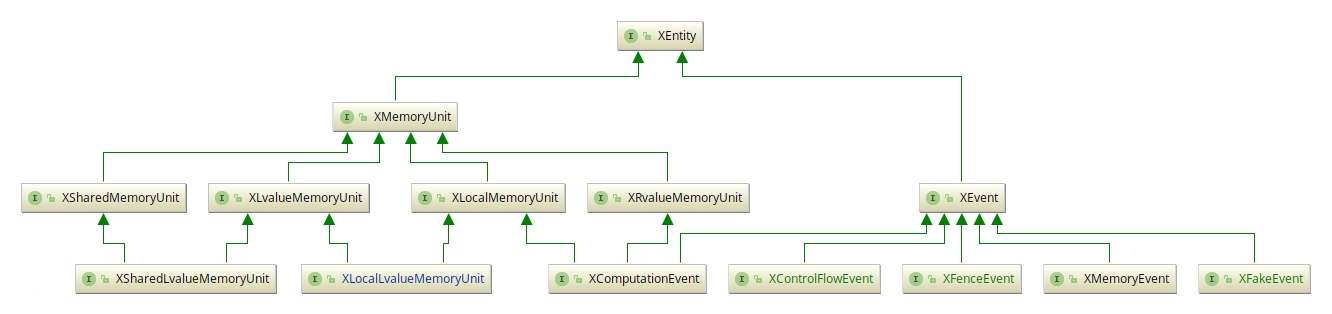
\includegraphics[width=\textwidth,keepaspectratio]{img/my/class-diagrams/XEntity-interfaces.png}
  \caption{The inheritance tree of interfaces of \xgraph{}}
  \label{fig:class-diagrams:XEntity-interfaces}
\end{figure}

All elements of \xgraph{} implement the interface \texttt{XEntity}.
There are two main kinds of X-entity: \textit{events} that implement the \texttt{XEvent} interface, and \textit{memory-units} that implement the \texttt{XMemoryUnit} interface.

Following the litmus tests format, we distinguish three types of \xgraph{}: one for a process, one for a litmus-initialisation block and one for the assertion statement.
However, all three types of the \xgraph{} are modelled by the same graph structure \texttt{XProcess} with certain restrictions complied by the corresponding type of X-interpreter that constructs the graph. %TODO: rename to XThread ?
This simplifies drastically the processing of different types of code blocks as they all are modelled by the same data structure.
The examples of restrictions on X-graphs are the following: the initialisation block can not have branchings, fence events; the process cannot have assertion events; the assertion block can not have shared-memory events or fence events.
We discuss the interpretation of different types of statements in more detail in Section~\ref{ch:impl:proc:x-compiler:compilation}.

\paragraph{Memory units}
\label{ch:impl:model:xgraph:mem}

The \textit{memory unit} is a memory cell of an abstract machine executing the code.
This machine has an infinite number of arbitrary-sized \textit{registers} (local memory units) and \textit{locations} (shared memory units).
Local memory units inherit the \texttt{XProcessLocalElement} interface, that stores the ID of the owning process.
Figure~\ref{fig:class-diagrams:XMemoryUnit} represents inheritance hierarchy of memory units.

%TODO!!! Remove watermark from the pictures!
\begin{figure}[t]%[!b]%[H]
  \centering
  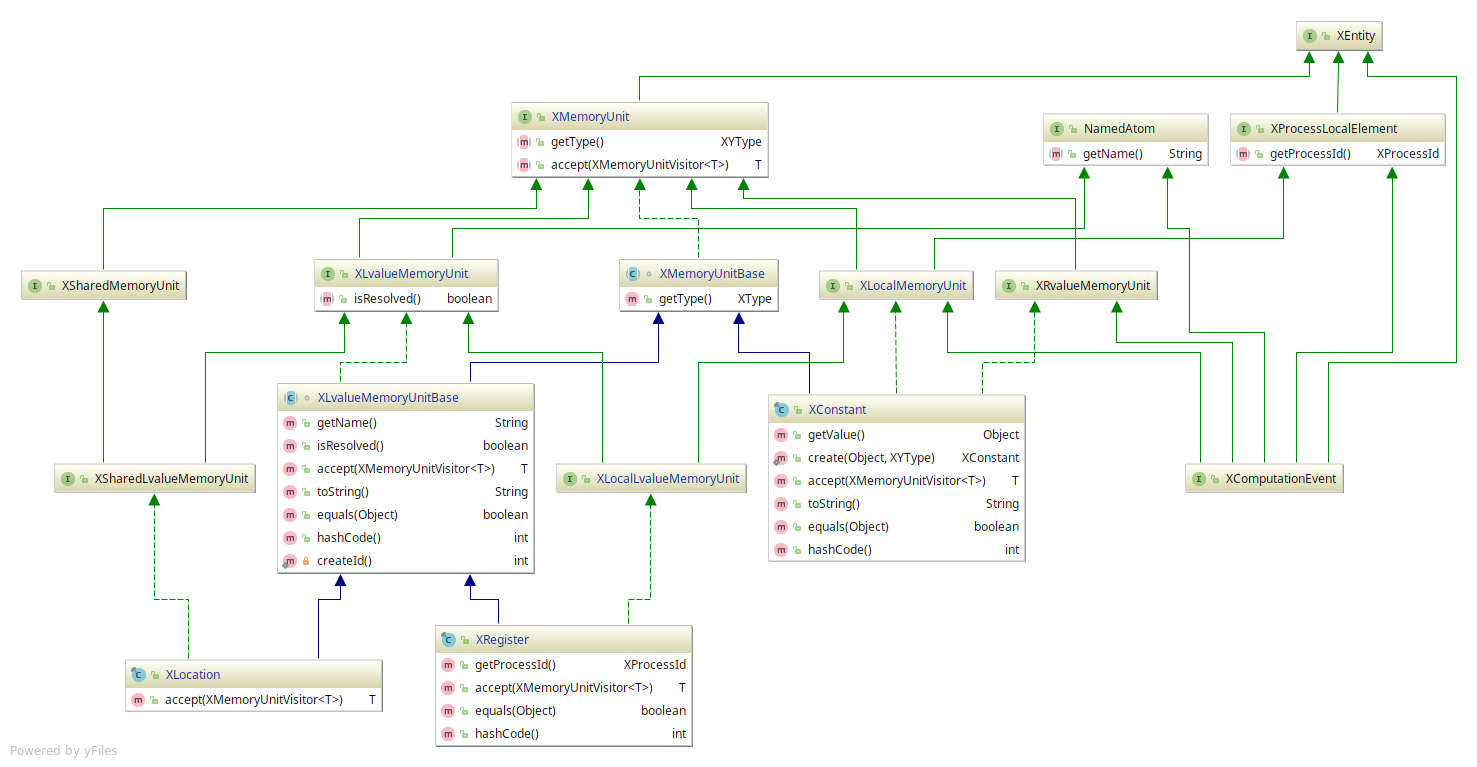
\includegraphics[width=\textwidth,height=\textheight,keepaspectratio]{img/my/class-diagrams/XMemoryUnit-m.png}
  \caption{The inheritance tree of \xgraph{} memory units}
  \label{fig:class-diagrams:XMemoryUnit}
\end{figure}

Following the terminology of the C standard, we distinguish the \textit{r-value} and \textit{l-value} memory units (unlike r-values, the l-values may be assigned a new value).
As r-values cannot change their value, they can be seen as the value itself (therefore the \texttt{XComputationEvent} is modelled as an local r-value memory unit, see more detailed discussion further in current Section).

Each memory unit has an \texttt{XType} associated with it.
The X-type is a symbolic representation of the C primitive type%
%
\footnote{Here we should note that \porthos[2] can eventually evolve to be able to analyse programs written in an OOP language (for instance, in C++). In this case, the \texttt{XType} will have more complex structure than a simple enumeration, which it has when we need to emulate only primitive types of C language. See more detailed discussion on input language type system in Section~\ref{ch:impl:proc:x-pre-compiler:type}.} %TODO!!!!! Check that XType is really a simple enumeration
%
that is easily convertible to an SMT-type (modelled as \texttt{ZType}).%TODO: add the class ZType
As the type of an X-memory unit may not be resolved correctly, the memory units keep this information as a boolean flag.

The memory units are created and stored by the \texttt{XMemoryManager}, which provides interface for accessing memory units during compilation stage.
For more detailed description of memory management see Section~\ref{ch:impl:proc:x-compiler:mem}.



\paragraph{Events}
\label{ch:impl:model:xgraph:evt}

An event (\texttt{XEvent}) represents the fact of executing the primitive operation, which is independent from other events.
Each event is specified by the process generated them and a unique event label.
This information is stored by events in the immutable structure \texttt{XEventInfo}.
Also, each event carries the reference to the Y-instruction that has generated it.

The following interfaces model basic kinds of events (see Figure~\ref{fig:class-diagrams:XEntity-interfaces}):
%\begin{itemize}[noitemsep]
\begin{outline}
  \1 \texttt{XMemoryEvent} \\
  The memory event defines the transfer of the value from one memory unit to another.
  There are four types of memory events (the arrow denotes the direction of the data-flow):
  %\begin{itemize}[noitemsep]
  \2 \texttt{XRegisterMemoryEvent}: \\
    $(\texttt{XLocalLvalueMemoryUnit}) \leftarrow (\texttt{XLocalMemoryUnit})$,
  \2 \texttt{XLoadMemoryEvent}: \\
    $(\texttt{XLocalLvalueMemoryUnit}) \leftarrow (\texttt{XSharedMemoryUnit})$,
  \2 \texttt{XStoreMemoryEvent}: \\
    $(\texttt{XSharedLvalueMemoryUnit}) \leftarrow (\texttt{XLocalMemoryUnit})$, and
  \2 \texttt{XInitialWriteEvent}: \\
    $(\texttt{XLvalueMemoryUnit}) \leftarrow (\texttt{XRvalueMemoryUnit})$.

  %\end{itemize}%TODO incompleted enumeration
  %TODO: either say st about getLoc(), getReg(), or remove them from code
  
  \1 \texttt{XComputationEvent} \\
  %TODO: say sth about how we not produce thousands of comput events
    We distinguish two types of computation events:
      %\begin{itemize}[noitemsep]
      \2 \texttt{XUnaryComputationEvent} that encodes bit negation and no-operation; and 
      \2 \texttt{XBinaryComputationEvent} that encodes numeric operations (such as addition, multiplication, etc.), bit vector operations (such as bit-and, bit-xor, etc.), relative operations (such as greater-then comparison, equality comparison, etc.), and logical operations (such as conjunction and disjunction). 
      %\end{itemize}
    \newline
    The computation event class implements both \texttt{XEvent} and \texttt{XMemoryUnit}.
    This is a model-level optimisation, which is possible because a computation event performs computation over local-only memory and does not change value of any memory unit.
    Thus, the \textit{computation} abstraction (as the CPU time spent for the computation itself) can be safely removed from the model, and the computation event can be seen as a zero-time operation that produces the \textit{value}.
    For analysing large expressions this optimisation is sensible because it considers the whole expression as a single computation event, encoded therefore as a single SMT-variable.
    \newline
    Note, for the purpose of simplifying the X abstraction level, computation events may have been modelled as invocations of bodiless functions (for instance, the operation `\lstinline{x + y}' may be modelled as the invocation of the function `\lstinline{+}' with the arguments \lstinline{x} and \lstinline{y}).
    However, current version of \porthos[2] maintains the \texttt{XComputationEvent} as the operators are supported by the SMT solver.
    
  \1 \texttt{XControlFlowEvent} \\
    The control-flow event indicates a non-linear jump in the code. We distinguish two kinds of control-flow events: 
    \2 \texttt{XJumpEvent} that performs no computation and no data operation, it can be safely removed from the model as an optimisation; and
    \2 \texttt{XMethodCallEvent} that models the function call with the \texttt{fastcall} calling convention (passing arguments in registers).
    %TODO: check the diagrams if the XMCE really inherits XLMU
    The function call also implements the \texttt{XLocalMemoryUnit} since it represents the computed value returned by the function call.
    If the function has been resolved, the actual arguments are bind to the formal parameters (treated as temporary local memory units), the called \texttt{XMethodCallEvent} is pushed onto the call stack, and the execution jumps to the function body.
    The call stack is bounded by the user-defined parameter; once the stack is full, the interpretation continues without jumping to the body of the invoked function (such cases are properly logged). %TODO: call-stack: user-defined parameter
    Each \texttt{return} statement creates the assignment of the function call event on the top of call stack.
    Note, this approach works for any kind of recursion, which is unrolled up the user-defined boundary as well as explicit loops.
    \\
    According to the Rice's theorem~\cite{rice1953classes}, in general case there always will be functions unresolved within an analysis launch.
    If the function has not been resolved, it can be safely assumed to be a no-operation function.
    In other words, we suppose that the knowledge base of \porthos[2] is complete and the tool can resolve all memory-operation functions and fence instructions.
    Although this can affect the completeness of the analysis, it is safe to make such an assumption as the user can check the log file and manually analyse the semantics of an unresolved call and it to the knowledge base if necessary.

  \1 \texttt{XFenceEvent} \\
    The fences are implemented as an enumeration \texttt{XBarrierEvent}.
    Current implementation of \porthos[2] supports all fences supported by \porthos{}: 
    \texttt{mfence}, %TODO: what about lfence and sfence from the x86fences.cat ?
    \texttt{sync}, \texttt{optsync}, \texttt{lwsync}, \texttt{optlwsync}, \texttt{ish}, \texttt{isb}, and \texttt{isync}.%TODO: description of each!
    
  \1 \texttt{XFakeEvent} \\
    The fake events are the auxiliary elements of \xgraph{}.
    %\begin{itemize}[noitemsep]
    \2 \texttt{XEntryEvent}, the per-process unique source event in the event-flow graph,
    \2 \texttt{XExitEvent}, the process sink event,
    \2 \texttt{XNopEvent}, the no-operation event (a jump to the next event), used for correct encoding in case when the control-flow branch does not have any event (see Figure~\ref{encode:branching:nop}), and
    \2 \texttt{XAssertionEvent}, the reachability assertion made at the postlude statement of the program.
    An assertion is modelled as an event for the purpose of encoding the postlude statement as a separate process that is compatible with the encoder.
   % \end{itemize}
%\end{itemize}
\end{outline}

%TODO: say about IDs from old code


\paragraph{Edges}
\label{ch:impl:model:xgraph:edges}
As the graph is represented by an adjacency matrix, its edges are stored in (immutable) hash-maps.
We distinguish the following kinds of edges:

\begin{outline}%[noitemsep]
  \1 the \textit{control-flow edges}:
    \2 the \textit{primary edges}, that denote both $\epsilon$-labelled transitions (in case of linear sequence of events) and conditional transition that evaluates the conditional event (the source of the transition) to the \textit{true}, and
    \2 the \textit{alternative edges}, that denote conditional transitions for which the conditional event (the source) was evaluated to the \textit{false}; and
  \1 the \textit{data-flow edges}:
    \2 the \co{}-relation edges, and 
    \2 the \rf{}-relation edges.
\end{outline}


\paragraph{Graph invariants}
\label{ch:impl:model:xgraph:invariants}
Once being constructed, the graph must conform the following requirements (see also Section~\ref{ch:enc:bmc:cf}):

\begin{enumerate}[noitemsep]
\item the graph must have a single source with no ingoing edges, and two sinks of different kinds without outgoing edges,
\item the graph must be connected,
\item each node of the graph can have either one or two direct control-flow successors,
\item only nodes of type \texttt{XComputationEvent} can have two direct control-flow successors,
%\item each node except the source node must have at least one parent
\item a \co{}-edge connects two writes, an \rf{}-relation edge connects a write and a read,
\item all write-event nodes except initial write-nodes must have exactly one \co-predecessor, and
\item all write-event nodes except final write-nodes must have exactly one \co-successor.
%TODO: \item \textbf{TODO: more?}
\end{enumerate}

%\paragraph{Graph builder} % TODO: in code: remove graph hierarchy by combining unrolled and normal. Add a bool 'UnrolledStatus' -- thus we can keep genericity
%\label{ch:impl:model:xgraph:builder}
%TODO: code : NOTE: 'FlowGraph<N extends FlowGraphNode>' may be just 'FlowGraph<N>'


%\paragraph{Graph example} %(in 5_eval.tex)
%\label{ch:impl:model:xgraph:example}

%hashcode, uniqueness

%\lstinputlisting{inc/XEventVisitor-cleaned.java}

\subsubsection{W-model}
\label{ch:impl:model:wmodel}
%TODO: almost not implemented !

The \textit{\wmodel{}} represents a recursive AST of \textit{computations over relations} and assertion expressions defined by the memory model.
The atomic elements of \wmodel{} are the basic relations (\po{}, \rf{} and \co{}; see Section~\ref{ch:wmm:model:relations}) and sets of events ($\mathbb{R}$, $\mathbb{W}$, $\mathbb{IW}$, etc.; see Section~\ref{ch:wmm:model:events}).
The expressions of \wmodel{} are unary (such as complement, transitive closure, etc.) and binary operations (such as union, intersection, etc.) over relations or sets of events; see Section~\ref{ch:wmm:cat}.
For the sake of transparency, each element of a \wmodel{} contains the origin location as the coordinates of the string in the model file. %TODO: implement origin for w-model

%todo: enumerate elements -- after refactoring>


%todo: rename everywhere assertions <- axioms


\subsubsection{Z-formula}
\label{ch:impl:model:zformula}

%TODO: not implemented at all !

The \textit{\zformula{}} representation is a wrapper for an SMT-formula used as an additional abstraction level used to increase the transparency of the architecture, simplify the debugging process and ease the support of different SMT solvers.
As all other internal representations, the \zformula{} is implemented as an immutable data structure.

The Z-abstraction level models the the logical formulas (definitions and assertions) that are put on the assertion stack of the SMT solver.
Generally, a \zformula{} represents the S-expression-based syntax of the SMT-LIB language~\cite{smt-lib}. % the semantics of SMT-LIB formulas defined in~\cite[Chapter 5]{smt-lib}.
Currently, the \zformula{} supports definitions and assertions over \textit{variables} and binary and unary \textit{expressions}.
However, in future it may be extended to support \textit{function symbols} and \textit{binders} (existential and universal quantification, pattern matching and functional type construction).

All expressions of a \zformula{} are \textit{typed} (or \textit{sorted}, in terms of SMT-LIB standard).
Basically, we distinguish \textit{boolean} and \textit{numeric} (integer, bitvector, real) expressions.
The typing of a \zformula{} is necessary for checking the basic validity of its expressions and converting it to a typed SMT-LIB formula.
For the sake of transparency, each element of a \zformula{} contains the origin location as the reference to the X-element that produced current Z-element. %TODO: implement origin for z-formula

%todo: enumerate elements -- after refactoring>


\subsection{Processing units} %Transformation}
\label{ch:impl:proc}

%todo: after all, list HERE which modules (classes, managers) are being initialised during the pre-compilation. I'ts good to have the dependencies graph on moduls (operational semantics:) )

This section describes program units that construct, transform and analyse internal representations described before. % steps of construction of the program representations and transformations applied to them.
We assign unique numbers to the processing units, which can checked in Figure~\ref{fig:arch} (within gears depicted in the top-left corner of each processing unit).
%Further in current Section, the subsection titles have a number in parentheses, which correspond to a unique number of the  processing unit being discussed.
%These numbers are pictured within the gear in the top-left corner of each processing unit in Figure~\ref{fig:arch}.
%he numbers in parentheses correspond the numbers of processing units pictured within gears in Figure~\ref{fig:arch}.

The construction of the \xgraph{} is performed in three stages.
First, the \ytree{} is compiled to a \textit{cyclic} control-flow event-based graph \xgraph[CF].
Then, this graph is unrolled to an \textit{acyclic} control-flow event-based graph \xgraphU[CF].
After that, the compiler is able to perform the data-flow analysis and produce the full event-based graph \xgraphU[CF+DF], which remains to be \textit{CF-acyclic} (no cycles among control-flow edges).

Most data structures are processed by units that implement the \textit{visitor} pattern~\cite{palsberg1998essence}.
This is a behavioural pattern that separates the program logic from the object implementation by specifying handling methods for each element of the object.
The general structure of the visitor pattern is illustrated by the pseudo-java code in Figure~\ref{fig:visitor}.
The visitor pattern performs the double-dispatching, a mechanism for decreasing the cohesion between the DTO (the visitee) and the processor class (the visitor): the visitee implements the \textit{accepting} method that gets the visitor as an argument and invokes its \textit{visiting} method with itself as an argument.
Thus, the method call resolution is performed statically at compile-time without any overhead at run-time.
%To visit an instance \lstinline{x} by a visitor \lstinline{v}, the program should call the accept-method of \lstinline{x} and pass \lstinline{v} as an argument.
In our implementation, the visitor (not the visitee) cares about the continuation of traversing its children.

\begin{figure}[h]
\centering
%\begin{multicols*}{2}
\begin{minipage}[t]{.55\textwidth}
\begin{lstlisting}[language=java]
interface Element {
  <T> T accept(Visitor<T> visitor);
  ...
}

class AnElement implements Element {
  @Override
  <T> T accept(Visitor<T> visitor) {
    return visitor.visit(this);
  }
  ...
}
\end{lstlisting}
%[* \vfill\null \columnbreak *]
\end{minipage}% <---------------- Note the use of "%"
\begin{minipage}[t]{.45\textwidth}
\begin{lstlisting}[language=java]
class Visitor<T> {
  T visit(AnElement e) {
    // visiting logic
    ...
    // continue recursively
    e.getChild().accept(this);
  }
  T visit(AnOtherElement e) {
    ...
  }
  ...
}
\end{lstlisting}
%\end{multicols*}
\end{minipage}
\caption{Illustration of the visitor pattern}
\label{fig:visitor}
\end{figure}

We consider the visitor pattern as the most natural way for operating the hierarchical data structures such as AST.
However, we use its double-dispatching capabilities to reduce cost of multiple type casting performed while traversing the elements of a non-recursive data structure.
The operator instance, instead of having a single method that handles and element of the instance, extends the visitor interface and splits the handler method into multiple methods, one for each type of element.

For traversing graph data structures, we mostly follow the \textit{iterator} pattern: the special object \texttt{Iterator}, that has access to elements of the data structure, iterates over them in some order (for example, in topological order as it is implemented for \xgraph{}).
%Since in \porthos{} we usually do not need to browse an object elements in different order, the iterator creation is performed by the data structure itself.
%However, in contrast to the visitor pattern, the visitor of a plain data structure should be used with an \textit{iterator} that has access to the elements of the object and passes them to the visitor.
The construction of immutable data structures is performed by units that follow the \textit{builder} pattern.
A builder is a mutable object that contains methods "filling" it by the elements that will constitute the result complex object.
The methods contain basic validity checks of the elements.
Once a builder has been built, it cannot be modified.


% todo: test pre-/post-fix operations //+think how current tool will behave if there's more than one post-operation //and pre-operation

\subsubsection{Input parsers}
\label{ch:impl:proc:input-parser}

Both input-language and input-model parsers are implemented via \tool{ANTLR} parser generator.
%In Figure~\ref{fig:arch}, the input parsers are denoted as (1) and (2) processing units.
Details on the input program language grammar are discussed in Section~\ref{ch:impl:input}.
Currently, \porthos[2] does not consider preprocessor instructions (it ignores them).
For implementing the inter-procedural mode of \porthos{}, it is crucial to support inclusion of header files (the \texttt{\#include} preprocessor directive).
Next step would be implementing the support of macros and conditional compilation directives, that are used often in C code.
As preprocessor statements may appear in arbitrary place of a program, the preprocessor must be a stateful processing unit that reads the token stream and dynamically instrument the program by interpreting directives and expanding macros.
%The \tool{ANTLR} grammar for the C preprocessor may be found 
%more macros (stateful) : https://gcc.gnu.org/onlinedocs/cpp/Macros.html

The input memory model language \cat{} is discussed in Section~\ref{ch:wmm:cat}.
The \tool{ANTLR} grammar for \cat{} language was extracted from the parser used by \tool{herd} tool%
%
\footnote{The \tool{herd} project repository: \url{https://github.com/herd/herdtools7}} %
%
written in OCaml.
%TODO: upload the grammar to github
%The input memory model 
%TODO: add reference to the grammar file in github repository OR include a short version as an appendix}

%todo: maybe: move something from the input language chapter here


\subsubsection{W-model constructor}
\label{ch:impl:proc:w-constr}

%TODO: <not implemented yet>
The \wmodel{} representation is constructed by the stateless visitor \texttt{Cat2WmodelConverterVisitor} from the ANTLR syntax tree \texttt{CatParser.MainContext} of the memory-model defined in \cat{} language.
%In Figure~\ref{fig:arch}, the \wmodel{} constructor is denoted as the (3) processing unit.
Currently, the visitor supports the small subset of \cat{} language, which constitutes only non-functional declarative expressions of the language as the support for functional-style expressions requires implementing the full OCaml interpreter.
However, some most commonly used functional-style expressions may be supported by mapping them syntactically to corresponding W-elements by the \wmodel{} constructor.

Following the principle of transparency, the \wmodel{} constructor aborts its work with the \texttt{NotSupportedException} if met the unrecognised syntax construction (in contrast to the \porthos[1] approach in which the \texttt{null} value was produced in all exceptional states).

%todo: file tree of w-model to appendix -- after code fixing>


\subsubsection{Y-tree constructor}
\label{ch:impl:proc:y-constr}

The \ytree{} is constructed by the stateless visitor \texttt{C2YtreeConverterVisitor} from the ANTLR syntax tree \texttt{C11Parser.MainContext} of the C language.
As the \wmodel{} constructor, the \ytree{} constructor aborts its work with the \texttt{NotSupportedException} once it meets an unsupported syntax construction.
%TODO: Rename YConverterException <- YParserException
A syntax exception \texttt{YConverterException} is thrown if the converted syntax tree contains semantic errors that prevent it to be converted to the \ytree{}.

As a \ytree{} constitutes a generic AST, the \ytree{} constructor expands the syntactic sugar expressions and statements (for example, a \texttt{switch}-statement is converted to the equivalent \texttt{if}-statement).


\subsubsection{X-graph pre-compiler}
\label{ch:impl:proc:x-pre-compiler}

The precompiler traverses the \ytree{} and collects information necessary for its compilation into an \xgraph{}.

%TODO: not supported yet


\paragraph{The label resolution}
\label{ch:impl:proc:x-pre-compiler:label}

%TODO: <not implemented yet>

The label resolution is necessary for establishing links to labelled statements. %a process of linkage the text labels referenced in code to the places of their declaration.
In C, labelled statements are declared via the colon-syntax `\texttt{<label>\;:\;<statement>}', and the labels are referenced by the jump-statement `\texttt{goto\;<label>}'.
The label resolution algorithm traverses the \ytree{} and collects all declared labels into a map that points a label to the labeled statement. %TODO: code: remove temp label generation, it's stupid. put null.
This information is used during compilation to set up unconditional jumps.


\paragraph{Type analysis}
\label{ch:impl:proc:x-pre-compiler:type}

C language has a static (resolved at compile-time) manifest (all types are declared explicitly) type system.
Comparing to languages that use type inference, the type analysis of a C program constitutes a simple propagating the type information (obtained from variables declarations) to all expressions. % according the rules of propagation. For example, 
Being carried at Y- and X- representation levels, the type is converted to a~Z-type at the stage of the Z-formula encoding (see Section~\ref{ch:impl:proc:z-encoder}).

%TODO: YOU REALLY NEED TO THINK MORE ABOUT TYPES ON Y, X, Z LEVELS + reconsider this paragraph (and others about types)
Currently, \porthos[2] handles only the primitive C types (such as \texttt{int}, \texttt{char}, \texttt{float}, etc.), which is modelled as an enumeration \texttt{XType}. %TODO: model it.
The array dimension is stored at the Y-level as an integer number (currently this information is not used as \porthos[2] does not support arrays, although this information can be used at the stage of pre-compilation for converting array elements to separate variables). %the array operations are converted to ).
In addition, \porthos[2] has a built-in extensible database storing the semantics of non-primitive C types stored by the \texttt{X2ZTypeConverter}, %TODO: Or XTypeHookManager?
which can be requested for converting an X-type to a~Z-type. %TODO: implement this.
%TODO: describe the XType (before) + implement this clearly! + definitely get rid of bit32

%TODO: <not implemented>
The type analysis algorithm should consider the type aliases supported by C language (defined by the \texttt{typedef} instruction).
For resolving the type aliases, the precompiler should make an extra traverse of the \ytree{} before the pre-compilation stage and build up a symbol map.

%TODO: <not implemented>
The type analysis also includes the process of resolving semantics of function invocations.
The result is stored in a map of invocation expression to the resolved function signature, so that the compiler can decide either to jump to the function body and interpret it, or to hook the invocation if the semantics of the function is resolved.
However, due to lack of polymorphism and function overloading mechanism inherent to OOP languages, the function resolution algorithm may set up the mapping only for the function name and thus may neglect analysis of types of the arguments, we build the mapping for the full function signature so that the type analysis preprocessing unit may be used for analysing the C++ code if needed.

%TODOOOOOOOOOOOOOOOOOOOOOOOOOOOOOOOOOOOOOOOOOOOOOOOOOOOOOOOOOOOOOOOOO
%The X-type construction: \textbf{TODO} //code of class YType2TypeConverter (todo: rename: it's not conversion, it's a type construction, from the y-level name+qualifiers+
%- on Z level, type is one-pointer-level
%- The typification algorithm: propagation rules for each of Y
%- as vector array as needed.
%%
%Y: quantifiers+specifiers+typeName
%X: ?.. Z? TODO: rename+rework XType->XZType
%Z: Int, Real, Boolean, BitVector[N]


\paragraph{Variable kind analysis}
\label{ch:impl:proc:x-pre-compiler:var}

On the compilation stage, once the compiler meets the reference to a variable, it should know whether it refers to a local or global variable.
The kinds of variables have to be determined on the pre-compilation stage.

%\vspace{1em}
The following types of variables are detected as \textit{global variables}:
%TODO: not implemented
\begin{itemize}
\item a variable was declared as a pointer;
\item a variable whose address was accessed by any process;
\item a variable that was declared as a parameter of the process function; and
%TODO: say sth about KERNEL ANALYSIS MODE BEFORE !!!!!!!!!!!!!!!!!!!!!!!!!!!!!!!!!!!!!!!!!!!!!!!!!!!!!!!!!!!!!!!!!!!!!!!!!!!!!!!!!!!!!!!!!!
\item a variable that was exported by the \texttt{extern} keyword (in the kernel-analysis mode, the functions \texttt{EXPORT\_SYMBOL} and \texttt{EXPORT\_SYMBOL\_GPL} also export symbols for dynamic linking). %https://lwn.net/Articles/154602/
\end{itemize}


\subsubsection{X-graph compiler}
\label{ch:impl:proc:x-compiler}

The X-compiler is the main component that transforms the recursive \ytree{} data structure to the plain \xgraph{} representation.
It is a complex processing unit; Figure~\ref{fig:compiler} illustrates the relationship between the principal components of the X-compiler in the UML language.

\begin{figure}[!t]%[H]
    \centering
  %draft=true
  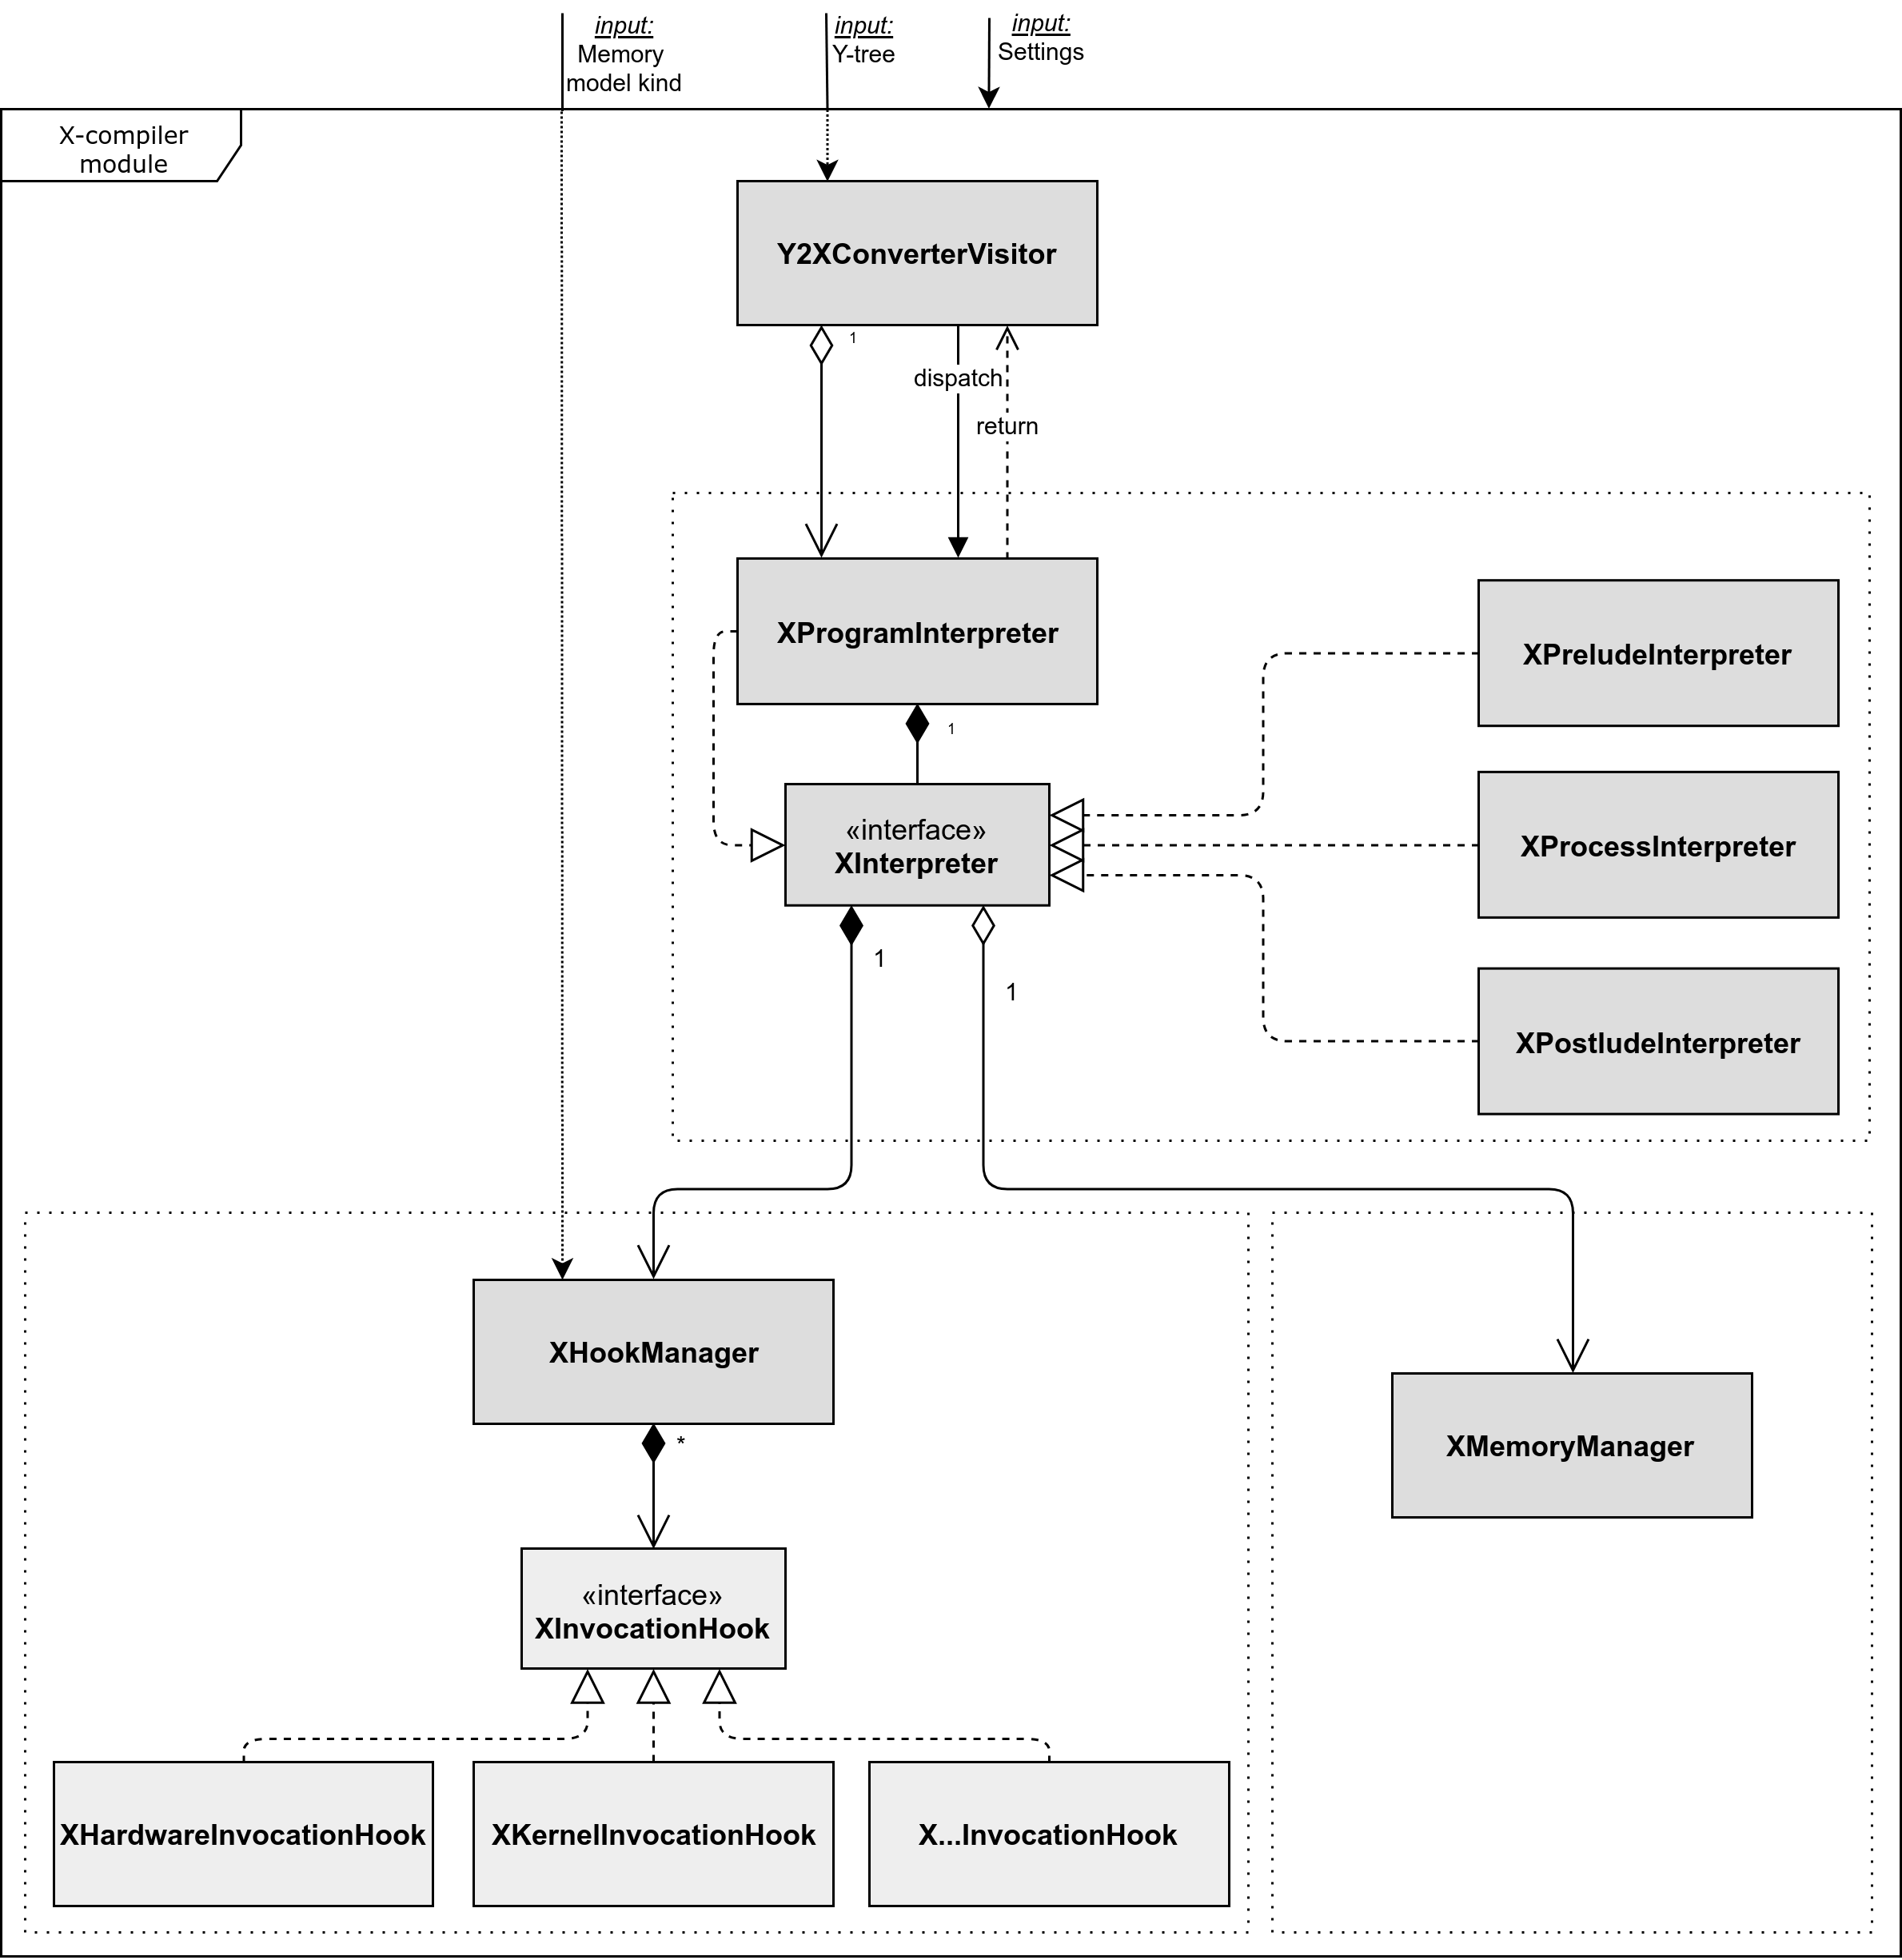
\includegraphics[max width=\textwidth,keepaspectratio]{img/my/draw.io/X-compiler.png}
  \caption{Main components of the X-compilation processing unit}
  \label{fig:compiler}
\end{figure}

The main class representing the X-compiler is \texttt{Y2XConverter}. %TODO: draw it on Figure.
It receives as input the \ytree{}, the memory model kind and user settings (for instance, the interpreter mode defining the set of invocation hooks enabled during the analysis run).
The \texttt{Y2XConverter} creates an instance of the stateless visitor \texttt{Y2XConverterVisitor} that traverses the \ytree{} while invoking the stateful interpreter \texttt{XInterpreter}.
The \texttt{XInterpreter} carries the \xgraph{}-builder and provides \textit{action} methods for changing its state and thus the filling in the builder.
The interpreter requests the managers such as \texttt{XMemoryManager}, \texttt{XHookManager}, \texttt{XTypeManager} for additional information. 

We distinguish three types of processes (each implementing the \texttt{XInterpreter} interface):
\begin{itemize}[noitemsep,topsep=0pt]
\item the prelude process \texttt{XPreludeInterpreter} (to be executed before all other processes) that allows only declaration of local or shared variables, computations and memory operations;
\item the postlude process \texttt{XPostludeInterpreter} (to be executed after all other processes) that allows only declaration of local variables, memory operations, computations and assertions;
\item the process \texttt{XProcessInterpreter} (to be executed in parallel) that allows all X-compiler interface operations except declaration of shared variables %(that should be declared during pre-compilation stage or during compilation of the prelude process)
and program assertions (i.e., it allows declarations of local variables, computations, barriers, unconditional jumps, non-linear branching statements, and method calls).
\end{itemize}

As the prelude process can declare shared variables, its compilation must go first.
%TODO: think about sorting processes at the pre-compilation stage
The first event of each process must be the \texttt{XEntryEvent} and the last events must be events of type \texttt{XExitEvent}.


\paragraph{Memory manager}
\label{ch:impl:proc:x-compiler:mem}

The \xgraph{} abstract machine model disposes infinitely many memory units, both local and shared (see Section~\ref{ch:impl:model:xgraph:mem}).
The X-compiler accesses all memory units via the \texttt{XMemoryManager}, which by the end of pre-compilation stage is already initialised (has registered all shared memory units).
However, the memory manager is a stateful component of the compiler as it offers the methods for declaring and removing local memory units dynamically at the compilation time.

The interface methods exposed by the \texttt{XMemoryManager} are presented in Figure~\ref{fig:mem-manager}.
At each time of the compilation process, the \texttt{XMemoryManager} can resolve the memory unit by its name.
Following the C standard, local memory units have higher priority over global ones (the method \texttt{getDeclaredUnitOrNull} returns the first memory unit found, either a global one or a local one, or null if no memory units with requested name have been registered).
Since C language allows usage of variables that have the same name to be declared in nested contexts, the \texttt{XMemoryManager} carries the stack of block contexts for local variables. %TODO: refactor XMemoryManager! 

\begin{figure}[h]
\centering
\lstinputlisting[language=java]{inc/lst/XMemoryManager.java}
\caption{X-memory manager public interface}
\label{fig:mem-manager}
\end{figure}


\paragraph{Invocation hook manager}
\label{ch:impl:proc:x-compiler:hooking}

%TODO: cite again here : alglave2018frightening + other Kernel references

%MethCallE : bind parameters with values (load them to temp registers) + remember the return-register
%reutrn event= assign the return-register + simple jump

The invocation hooking module serves as a knowledge base that stores the semantics of functions.
%TODO: rename HookManager -> XHookManager
Once the X-compiler meets the function invocation, it calls the \texttt{XHookManager}, which tries to match the function signature (in the case of program in C language -- only the function name) across all signatures it stores.
If the signature matches, the hook manager intercepts the function call and interprets the hook action instead of invoking the function directly.
%TODO: say sth about the mode
The hook manager operates multiple invocation hooks depending on the user-defined mode.
All invocation hooks implement the interface \texttt{XInvocationHook}.
The result of an invocation hook interception is the \texttt{XInvocationHookAction}, a delayed operation implemented on the top of lambda functions of Java.
The hook action is invoked with actual arguments and returns an arbitrary \texttt{XEntity} as the result of invocation.

Current version of \porthos[2] contains two invocation hooks, the \texttt{XPorthosInvocationHook} for describing the compatibility-mode functions of the input \porthos[2] input language, and \texttt{XKernelInvocationHook} for describing the Linux kernel-specific functions.
An invocation hook can model any type of operations (memory, fence, computational, etc.).
For instance, the \texttt{XPorthosInvocationHook} intercepts calls \texttt{`location.store(atomic,register)'} and processes the store operation with respect to the specified atomic.
%TODO: more about described functions
%TODO: rename InvocationHook -> XInvocationHook

%TODO: kernel's : ACCESS_ONCE() access may be modeled as a volatile memory_order_relaxed access.  %http://www.open-std.org/jtc1/sc22/wg21/docs/papers/2015/n4374.html

% + RCU %https://www.kernel.org/doc/Documentation/RCU/whatisRCU.txt


\paragraph{Interpreter}
\label{ch:impl:proc:x-compiler:compilation}

%In this paragraph we discuss only the implementation of the process interpreter \texttt{XProcessInterpreter}.
%This interpreter is used to build the branched event-flow graph with all kinds of jumps, memory operations and fences.
The X-program interpreter is invoked by the \texttt{Y2XConverterVisitor} which walks down the recursive syntax tree \ytree{}.
The calls to the X-program interpreter are dispatched to currently maintained X-process interpreter.
To be able to properly recognise nested statements of the \ytree{}, the X-process interpreter needs to have stacks.
On any semantic error, the X-interpreter throws an \texttt{XInterpretationError}.

The interface methods of the \texttt{XInterpreter} are presented in Appendix~\ref{apx:xinterpreter}.
Note the clear modular independence of the X-interpreter as it has no methods that operate entities of the Y-level (all conversion work with Y-entities is done by the \texttt{Y2XConverterVisitor}).

All interface methods can be divided into two groups.
The first group constitute methods that emit events.
These methods construct an event object (as events contain the \texttt{XEventInfo} structure that stores information about the owning process, all events must be created by the process constructor, i.e. X-interpreter) and change the state of interpreter considering the newly created event.
Note that the methods \texttt{createComputationEvent} do not emit a computation event but only create one.
This is performed as optimisation that removes unused computations from the model (otherwise, for instance, the assignment 
`\texttt{x = 1 * (2 + 3)}' would be compiled to two consequent events `\texttt{eval(2 + 3); write(register <- eval(1 * eval(2 + 3)));}' instead of a single event `\texttt{write(register <- eval(1 * eval(2 + 3)));}').
If the computation event was not used at all (for example, in the following C code: `\texttt{foo(); 1; bar();}' the execution event `\texttt{eval(1)}' is skipped by the model), it is also removed from the event-graph (see justification in Section~\ref{ch:impl:model:xgraph:evt}).
The second group of X-interpreter methods consists of the methods for defining non-linear statements (branchings and loops).
These methods change the state of the interpreter and set up additional non-linear control-flow edges.
%`\texttt{register = 1 * (location + 2)}' would be compiled to three consequent events `\texttt{load(temp\_reg\_1 <- location); eval(temp\_reg\_1 + 2); write(register <- 1 * (temp\_reg\_1 + 2));}',


As a high-level instruction (Y-level) may be compiled into a sequence of low-level instructions (for example, a computation that involves shared variables should firstly load them into the local memory and then process the computation event over local-only memory), the interpreter must maintain the \textit{stack of contexts} and remember the \textit{previous event} to be able to correctly process nested non-linear statements of C language.
The context is a data structure that carries the \textit{state} and some additional information in the case of processing non-linear statements (e.g., conditional event, first and last then- and else-branch events for binding, etc.).
Once the new event has been emitted, the interpreter sets up control-flow edges w.r.t. state of the context on the top of the stack (the context stack is always non empty: the bottom context is a linear one).
The context state is an enumeration of the following values:
\begin{itemize}
\item \texttt{WaitingAdditionalCommand}: the interpreter is in the state of defining the complex (non-linear) statement and is not able to process any new event (will throw an exception if any) until the state is not changed;
\item \texttt{WaitingFirstConditionEvent}: the first next emitted event will be accepted as the first event of the condition evaluation (later, the loop edges will be set to this event);
\item \texttt{WaitingLastConditionEvent}: the next event must be of type \texttt{XComputationEvent}; it will be saved as the conditional branching event;
\item \texttt{WaitingFirstSubBlockEvent}: the first next emitted event will be accepted as the first event of the branching statement (later the interpreter will set up jumps to that event);
\item \texttt{WaitingNextLinearEvent}: the standard interpreter state for processing next linear event, and
\item \texttt{Idle}: the interpreter does not set up the edge from the previous event to the new event.
\end{itemize}

Each new event emitted by the interpreter is processed considering the state of the context stack:
the interpreter iterates over the context stack and sets up the edges by the graph builder depending on the state of each stack.
The state \texttt{WaitingFirstConditionEvent} is necessary for correctly interpreting the branching conditions, which shared variables are involved in.
If the non-linear statement is a loop statement, the loop back-edges will be set to this event.

Once interpretation of the (non-linear) branch is completed, its non-linear context is being popped out of the context stack (by interpreter method \texttt{startBlockBranchDefinition}) and added to the queue of \texttt{almostReadyContexts}.
The almost-ready-context becomes a ready-context (i.e., it moves to the queue \texttt{readyContexts}) once the non-linear statement definition has finished (the method \texttt{finishNonlinearBlockDefinition}).

Before processing a newly emitted event, the interpreter checks whether the queue \texttt{readyContexts} is not empty.
If so, it iterates over all ready-contexts and sets up control-flow edges considering that the newly emitted event is an exit-event" of the non-linear context (e.g., for a branching context the interpreter adds primary edges from condition-event to the first-true-branch-event and from the last-true-branch-event to the exit-event, the same is done with alternative edges for the false-branch).

%The \texttt{almostReadyContexts} queue is necessary for not adding erroneous edges on 

For the sake of simplicity of the interpreter, jump events (no-computation events) are present in the flow-graph, however they can be removed from it with rebinding ingoing and outgoing edges.


%algorithm for interpreting

%The method \texttt{tryConvertToLocalOrNull} makes an attempt to convert an arbitrary X-entity to the local memory unit: registers and computation events are casted and returned by the method as-is, shared memory units are copied to a temporary register (\texttt{declareTempRegister}), which is returned by the method.
%In other cases, the method returns \texttt{null}.

\subsubsection{X-graph unroller}
\label{ch:impl:proc:x-unroll}

In order to be encoded into an SMT-formula, the compiled graph needs to be acyclic~\cite{Porthos17b}.
To convert it to an acyclic form, we perform the \textit{unrolling} (sometimes called \textit{unwinding}) transfomation: each cycle is unrolled up to the user-defined bound $k$.
Comparing to \porthos[1], we have changed the meaning of the bound: instead of executing all cycles at most $k$ times, the \porthos[2] interprets the bound as the maximum number of events in the trace of the unrolled graph%
%
\footnote{The original specification of \porthos[2] stated that the unrolling bound $k$ must be interpreted as the maximum number of instruction in the original code (technically, the number of expressions in the ANTLR syntax tree).
Nonetheless, current implementation of the \xgraph{} unroller counts the X-level events as it is much simpler to implement (the questions about how to count complex expressions that involve multiple shared variables and method invocations are left open for the future versions of \porthos[2]).
For now, the information about the element of the ANTLR tree that corresponds to the X-event or Y-tree element is being lost during the transformations.
Instead, we use the \texttt{LocationService} discussed in Section~\ref{ch:impl:model:ytree} that in perspective may be extended for providing this information along with the text citation of the original code.}
%
.
The meaning of a bound was changed in order to increase predictability of the size of the result SMT-formula.
Not that recursive function calls create unconditional jumps back in the event-flow graph, which will also be recognised as a loop and be affected by the unrolling algorithm.

Considering the new meaning of the unrolling bound, the graph unrolling may be \textit{complete} (the loop has been executed a whole number of times) or \textit{incomplete} (the unrolling bound has triggered on not-the-last event of the loop), which can be modelled by two types of the sink events.
The user may need this information for understanding how the \porthos[2] interprets the cyclic program.
However, current implementation loses this information by having only one sink event.
Figure~\ref{fig:loop-unroll} illustrates the unrolling for the left-hand side cyclic control-flow graph (the square node $S_{+}$ denotes the complete sink node, and the $S_{-}$ denotes the incomplete sink).

%TODO: draw (and implement) diff types of exit nodes
\begin{figure}[t]
\centering
\resizebox{\linewidth}{!}{
\begin{tikzpicture}[->,>=stealth',shorten >=1pt,auto,node distance=1.5cm,semithick]
\node[c] (1) [] {$1$};
\node[c] (2) [below left of=1] {$2$};
\node[c] (3) [below right of=1] {$3$};
\node[c] (4) [below of=3] {$4$};
\path[->]
(1) edge [] node {} (2)
(2) edge [bend left=50,dotted] node {} (1)
(1) edge [] node {} (3)
(3) edge [] node {} (4)
(4) edge [bend right=80,dotted] node {} (1)
;
\node[draw=none] (impl) [right=3cm of 3] {$\overset{k = 6}{\longmapsto}$};
;
\node[c] (22) [right=3cm of impl] {$2_2$};
\node[c] (11) [above right=1cm and 1cm of 22]{$1_1$};
\node[c] (32) [below right=1cm and 1cm of 11] {$3_2$};
\node[c] (43) [below of=32] {$4_3$};
\node[c] (13) [below of=22] {$1_3$};
\node[c] (24) [below left=1cm and 1cm of 13] {$2_4$};
\node[c] (34) [below right=1cm and 1cm of 13] {$3_4$};
\node[c] (14) [below of=43] {$1_4$};
\node[c] (15) [below of=24] {$1_5$};
\node[c] (45) [below of=34] {$4_5$};
\node[c] (25) [below of=14] {$2_5$};
\node[c] (35) [below of=14] {$3_5$};
\node[c] (26) [below left=1cm and 1cm of 15] {$2_6$};
\node[c] (36) [below right=1cm and 1cm of 15] {$3_6$};
\node[c] (16) [below right=1cm and 0.2cm of 45] {$1_6$};
\node[c] (46) [below right=1cm and 0.3cm of 35] {$4_6$};
\node[rectangle,draw] (6inc) [below left=1cm and 3cm of 16] {$S_{-}$};
\node[rectangle,draw] (6com) [right=3cm of 6inc] {$S_{+}$};
\node[] (k1) [right=3.2cm of 11] {$(k = 1)$};
\node[] (k2) [right=1.7cm of 32] {$(k = 2)$};
\node[] (k3) [right=1.7cm of 43] {$(k = 3)$};
\node[] (k4) [right=1.7cm of 14] {$(k = 4)$};
\node[] (k5) [right=1.7cm of 35] {$(k = 5)$};
\node[] (k6) [right=1cm of 46] {$(k = 6)$};
\path[->]
(11) edge [] node {} (22)
(11) edge [] node {} (32)
(32) edge [] node {} (43)
(22) edge [] node {} (13)
(13) edge [bend right=10] node {} (24)
(13) edge [bend left=10] node {} (34)
(43) edge [] node {} (14)
(24) edge [] node {} (15)
(34) edge [] node {} (45)
(14) edge [] node {} (25)
(14) edge [] node {} (35)
(15) edge [bend right=10] node {} (26)
(15) edge [bend left=10] node {} (36)
(45) edge [] node {} (16)
(35) edge [bend right=10] node {} (16)
(35) edge [bend left=10] node {} (46)
(26) edge [bend right=10] node {} (6com)
(36) edge [bend right=5] node {} (6inc)
(16) edge [bend left=20] node {} (6inc)
(46) edge [bend left=20] node {} (6com)
;
\end{tikzpicture}
}
\caption{Example of the flow graph unrolling up to bound $k = 6$}
\label{fig:loop-unroll}
\end{figure}

The unrolling procedure is performed by the \texttt{XFlowGraphUnroller}. %, which extends the \texttt{FlowGraphDfsTraverser}
For unrolling the flow-graph, we perform the \textit{Deep-First Search (DFS)} while counting the Y-level instructions (for the unrolling bound) and keeping track of the depth stack (for detecting back edges needed for determining the type of sink node).
Also, during the unrolling each next event increments the \textit{unrolling depth counter} (the \textit{event reference-ID}) -- the integer that is stored by the \texttt{XEvent} thus making it \textit{an event reference} on non-zero values.
Each \texttt{XEvent} has the method `\texttt{XEvent asNodeRef(int refId)}' that clones the event-receiver with new value of reference-ID.
The methods \texttt{hashCode} and \texttt{equals} consider the reference-ID as the uniqueness field for all events except sink and source events (considering the usage of \texttt{HashMap} and Guava's \texttt{ImmutableMap} for storing events, proper setting of the hash-code methods is a crucial programming task).


%TODO!!!!!!!!!!! other schemes!\textsl{}
%During the work on \porthos[2], we have tested several different schemes of loop unrolling.


%- After we acquired the event-based representation, we can perform some modifications/simplifications/optimisations on it (separately, allowing user to manage them)


\subsubsection{X-graph data-flow constructor}
\label{ch:impl:proc:x-df}

Once the graph is unrolled, it can be augmented by data-flow edges.
As it was discussed in Paragraph~\ref{ch:impl:model:xgraph:edges}, the data-flow edges can represent either \rf{}- or \co{}-relation.
The \rf{}-edges join each write event to all read events that access the same location; the \co{}-edges join write events to the same location.

%TODO: why in old implementation we encode the negation of "co" ? same for "rf" above
%\url{https://github.com/hernanponcedeleon/Dat3M/blob/80341bec26021d41cf79eddc943e7cbe6f49322f/dartagnan/src/dartagnan/wmm/Domain.java#L204} >


\subsubsection{Z-formula encoder}
\label{ch:impl:proc:z-encoder}

The \zformula{} encoder transforms the program and the memory models to a single SMT-like representation.
It follows the encoding scheme described in Chapter~\ref{ch:enc}.
%TODO: say more!

\subsubsection{SMT-formula converter}
\label{ch:impl:proc:smt-converter}

As the \zformula{} follows the SMT-LIB standard, its translation to an SMT-formula constitutes almost one-to-one mapping.
The translation is performed by the stateless visitor \texttt{Z2SmtTranslator}.


\subsubsection{SMT solver}
\label{ch:impl:proc:smt-solver}
%TODO: check that we have ALL references in pre-word in this chapter
As it has been mentioned in Section~\ref{ch:impl:principles}, \porthos[2] uses the third-party SMT solver \tool{Z3}, which offers the Java API for constructing requests to the Z3 solver and interpreting its responses.


\subsection{Program output}
\label{ch:impl:out}

The result of execution of \porthos[2] is the verdict modelled by the class \texttt{AppVerdict}.
This is a structure that contains the result of analysis and auxiliary information such as collected errors and time of execution (separately for each stage of computing).
The app verdict may be rendered to any format convenient for the user.


%\subsection{Auxiliary components}
%\label{ch:impl:aux}
%
%\subsubsection{Watchdog timer}
%\label{ch:impl:aux:watchdog}
%
%%<not implemented>
%
%todo
%
%\subsubsection{Logger}
%\label{ch:impl:aux:logger}
%
%%<not implemented>
%
%todo


%todo: some words on necessity of contexts and lack of them. How would we implement them


%TODO: \section{Optimisations} 